% An extension of the article to include font size
\documentclass[10pt]{extarticle}
\usepackage[]{layout}
\setlength{\textwidth}{16cm}
\setlength{\textheight}{24cm}

\usepackage[T1]{fontenc}


\usepackage{helvet}
\renewcommand{\familydefault}{\sfdefault}
% \usepackage[helvet]{sfmath}
% \everymath={\sf}

\usepackage{parskip}

\usepackage[english]{babel}
\usepackage[left=2cm, right=2cm, top=2cm, bottom=2cm]{geometry}
\usepackage{afterpage}

 % Math packages
\usepackage{amsmath,amsfonts,amsthm}

\usepackage[pdftex]{graphicx}

% For hyphenation of texttt:
% https://tex.stackexchange.com/questions/299/how-to-get-long-texttt-sections-to-break
\usepackage[htt]{hyphenat}

% For syntax highlighting
\usepackage{minted}
\setminted[]{frame=single,fontsize=\small,samepage=true,breaklines=true,breakanywhere}

% Allow latex to play around with space stretching to prevent texttt's overflowing the page width
\setlength\emergencystretch{3cm}

\usepackage{xcolor}
\definecolor{linkcolor}{HTML}{000066}

% For links
\usepackage[hyphens]{url}
\PassOptionsToPackage{hyphens}{url}\usepackage[hidelinks = true, colorlinks = true, linkcolor = black, urlcolor = linkcolor]{hyperref}

% Fixing a pandoc related error
% https://tex.stackexchange.com/questions/257418/error-tightlist-converting-md-file-into-pdf-using-pandoc
\def\tightlist{}

% This allows using \Needspace{distance} to avoid subsections to start near the bottom of the page
\usepackage{needspace}

\usepackage{longtable}
\usepackage{booktabs}
\usepackage{caption}

% Adding breaklines=true to minted's settings seems to produce some errors related to fonts. This is
% the only fix that worked.
% https://stackoverflow.com/questions/70075331/pdflatex-file-cmss10-t3-cannot-open-type-1-font-file-for-read

\pdfmapfile{-mpfonts.map}

% Workaround for red boxes around @-signs in minted environments
% https://tex.stackexchange.com/questions/343494/minted-red-box-around-greek-characters
\makeatletter
\AtBeginEnvironment{minted}{\dontdofcolorbox}
\def\dontdofcolorbox{\renewcommand\fcolorbox[4][]{##4}}
\makeatother

% Increase table row height and make table border thickness consistent
\renewcommand{\arraystretch}{1.5}
\setlength{\arrayrulewidth}{0.75pt}

% REPORT FORMAT:
\begin{document}
\section*{Diverge-Converge Multi-Phase Audit
Model}\label{diverge-converge-multi-phase-audit-model}

\href{hans@cyfrin.io}{Hans Friese}, \href{patrick@cyfrin.io}{Patrick
Collins}, \href{alex@cyfrin.io}{Alex Roan}

\subsubsection*{Abstract}\label{abstract}

In this paper, we explore the shortcomings of current audit models and
present the Diverge-Converge Multi-Phase Audit (DC MPA), a novel
approach aimed at boosting the quality and efficiency of audits in the
Web3 sphere.

Our proposed audit model is structured into four essential distinct
phases: a traditional audit conducted by a lead (personal auditor or a
team of auditors or an audit firm), a public epochal time-boxed bug
bounty (PET bug bounty), an exclusive competition, and a final review.
Additional phases can be added according to the
protocol\textquotesingle s preference.

It is worth noting that the new model differs from a simple combination
of several single-phase audits. A unique feature of this model is how
each phase is interlinked with incentives and disincentives, fostering a
spirit of rigorous competition amongst auditors.

Being the first model of its kind to incorporate multiple distinct
phases of auditing, we anticipate that it will offer high-quality audits
and foresee its wide adoption in the Web3 space.

\section{Introduction}\label{1-introduction}

\subsection{Background}\label{11-background}

The Web3 realm, commonly hailed as the next generation of the internet,
is characterized by rapid evolution and expansion with many
decentralized applications and platforms. These decentralized networks
bring forth many advantages including enhanced privacy, resistance to
censorship, and a democratized platform for creating value.
Nevertheless, they also present unique security challenges that need to
be addressed.

The fabric of the Web3 ecosystem is woven with blockchain technologies,
smart contracts, and decentralized applications (dApps). Smart contracts
stand out as they form the backbone of many Web3 applications, defining
the rules and logic for decentralized interactions. Given their
self-executing nature and the fact that the actual code is publicly
available, smart contracts are highly susceptible to attacks and
exploits. The immutable nature of smart contracts also poses a
challenge, as any vulnerabilities in the codebase cannot be rectified
post-deployment.

According to the report from
\href{https://www.chainalysis.com/blog/2022-biggest-year-ever-for-crypto-hacking/}{Chainalysis},
\$3.8 billion was stolen in 2022. Major hacks and the affected protocols
are listed in \href{https://rekt.news/leaderboard/}{rekt.news}.

\begin{figure}[htp]
  \centering
  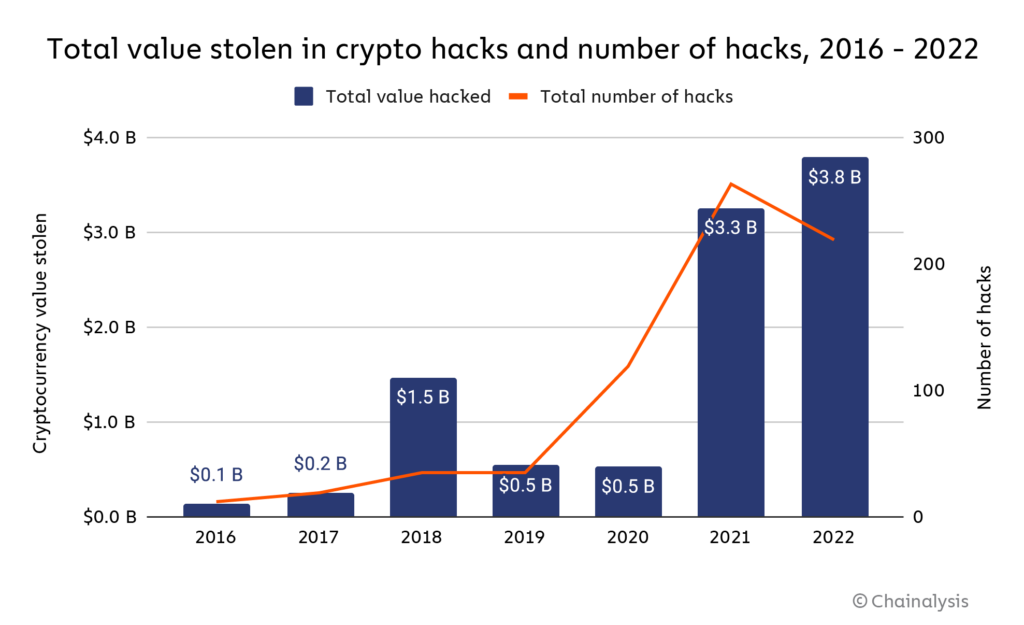
\includegraphics[width=10cm]{img/chart-hack-totals.png}
  \caption{\$3.8 billion was stolen in 2022}
  \label{fig:galaxy}
\end{figure}

The reality underscores the urgent need for comprehensive and robust
security audits in Web3.

Security audits involve scrutinizing the code of smart contracts to
detect and rectify vulnerabilities before deployment.

This paper explores the possible shortcomings of current audit models
and presents the Diverge-Converge Multi-Phase Audit Model, a novel
approach aimed at boosting the quality and efficiency of audits in the
Web3 sphere.

\subsection{Scope and Terminology}\label{12-scope-and-terminology}

This paper primarily focuses on the security aspects of smart contracts
and dApps within the Web3 ecosystem \textbf{prior} to their deployment.
Aspects related to the architectural recommendations during the
development and the post-deployment security are not within the purview
of this paper.

\begin{itemize}
\tightlist
\item
  The term "\textbf{protocol}" in this context denotes the smart
  contract or dApp that is the subject of the audit.
\item
  The "\textbf{client}" refers to the individual or organization that
  owns the protocol and commissions the audit.
\item
  An "\textbf{audit}" signifies inspecting the
  protocol\textquotesingle s code to detect and eliminate
  vulnerabilities. Generally the terms "audit" and "security review" are
  used interchangeably but we will use the term "audit" throughout this
  paper. In a narrow sense, we use the term "audit" to refer to the
  process of inspecting the protocol\textquotesingle s codebase that is
  ready to be deployed.
\item
  An "\textbf{auditor}" denotes the individual or organization entrusted
  with conducting the audit. Note that we use the term "auditor" to
  refer to the individual or organization that conducts the audit.
\item
  An "\textbf{audit report}" is the conclusive document the auditor
  produces upon completion of the audit process.
\item
  A "\textbf{bug bounty}" is a mechanism to encourage the public to
  discover vulnerabilities in the protocol. In a traditional bug bounty
  program, rewards are given only for the first reported instance of a
  particular vulnerability, with subsequent duplicate reports not being
  eligible for rewards.
\item
  A "\textbf{contest}" is a similar incentive-based process aimed at
  public participation in finding protocol vulnerabilities. Contrary to
  bug bounties, contests reward all valid vulnerability submissions.
\end{itemize}

\section{Defining a Good Audit
Model}\label{2-defining-a-good-audit-model}

In the context of Web3 application security, defining what makes an
audit "good" is a crucial discussion.

We suggest that an optimal audit model should meet three fundamental
criteria:

\begin{itemize}
\tightlist
\item
  Flawlessness, or \textbf{Perfectness}
\item
  Operational effectiveness, or \textbf{Efficiency}
\item
  The provision of supplementary benefits, which we categorize as
  \textbf{Plus}.
\end{itemize}

\subsection{Perfectness}\label{21-perfectness}

A high-quality audit aims for an ideal state we define as
\textbf{Perfectness}. Perfectness represents a scenario where the
audited codebase is entirely devoid of vulnerabilities. The quest for
perfectness makes the codebase progressively more secure and reliable as
we inch closer to this ideal state. The role of auditors is pivotal in
this journey - as they dig deeper into the code, unearthing and
resolving more bugs and vulnerabilities, the reservoir of potential
vulnerabilities diminishes. This ongoing cycle of discovering and
resolving vulnerabilities fuels a positive feedback loop in the audit
process. Each vulnerability spotted and fixed nudges us nearer to
perfectness, establishing a cycle of continuous enhancement toward a
secure codebase.

Pursuing audit perfectness encompasses two critical elements:
\textbf{Exploit Quality} and \textbf{Consult Quality}.

\begin{itemize}
\item
  Exploit Quality is a measure of the audit\textquotesingle s
  proficiency in detecting and evaluating potential vulnerabilities in
  the codebase. The objective is to unearth and address as many
  vulnerabilities as possible, reducing the remaining vulnerabilities
  and advancing towards perfectness.
\item
  Consulting Quality, on the flip side, refers to the
  auditor\textquotesingle s capacity to provide insightful advice and
  recommend best practices that enhance the overall security and
  robustness of the codebase, thus aiding the progress towards
  perfectness.
\end{itemize}

In this paper, we focus more on the exploit quality of the audit while
the consulting quality is also essential.

When addressing perfectness, multiple factors contribute to the quality
of the audit.

\begin{itemize}
\item
  Top-Tier Engagement Engaging auditors with relevant domain knowledge
  is crucial as their expert knowledge and experience significantly
  boost the exploit and consult quality of the audit.
\item
  Many Eyes The "Many Eyes" principle implies that having a larger pool
  of auditors reviewing the codebase can enhance the chances of
  identifying vulnerabilities.
\item
  Duration The duration of the audit can influence the audit quality. A
  longer duration allows auditors to conduct a more thorough review,
  discovering more vulnerabilities.
\item
  Number of Rounds The number of audit rounds can influence the audit
  quality. Conducting multiple rounds can lead to detecting and
  resolving more vulnerabilities, thus improving both the exploit
  quality and consult quality.
\item
  Synergy Collaborative brainstorming sessions between auditors and the
  protocol developers can enhance the audit quality. These sessions
  allow auditors to leverage each other\textquotesingle s expertise and
  share knowledge, leading to more comprehensive audits.
\item
  Tooling Advanced tools like static analyzers can automate certain
  parts of the audit, improving its efficiency and comprehensiveness.
\end{itemize}

\subsubsection*{The Role of Incentives and
Disincentives}\label{the-role-of-incentives-and-disincentives}

An essential consideration in auditing is the dedication of the auditor
due to the intensive nature of security audits. When we speak of
top-tier engagement, we\textquotesingle re referring to a review carried
out with high commitment.

This \textbf{Dedication} is a vital ingredient in a successful audit.
The auditor\textquotesingle s level of commitment can be influenced by
various factors, including but not limited to the incentives and
disincentives for the performance.

Ideally, a system should offer incentives or impose disincentives on the
auditor, influenced by specific "metrics". For example, an auditor could
be incentivized based on the number of vulnerabilities they uncover, or
face disincentives if they fail to adhere to set deadlines. This system
of incentives and disincentives is an integral part of the
Diverge-Converge Multi-Phase Audit Model, which we will delve into
later.

\subsection{Efficiency}\label{22-efficiency}

While striving for perfection is vital, it\textquotesingle s also
essential to maintain efficiency in terms of both turnaround time and
cost. A high-quality audit shouldn\textquotesingle t excessively delay
the protocol\textquotesingle s deployment or result in prohibitive
expenses, as these factors can hinder innovation and growth within the
Web3 ecosystem. It\textquotesingle s important to clarify that being
efficient doesn\textquotesingle t mean rushing deployment. Instead,
it\textquotesingle s about reducing time and cost while ensuring the
protocol\textquotesingle s security through thorough efforts. The
Diverge-Converge Audit Model is designed to enhance efficiency,
minimizing both the time and cost associated with completing an audit.

\subsection{ Plus}\label{23-plus}

A quality audit transcends mere perfection and efficiency, delivering
added value through services like:

\begin{itemize}
\item
  \textbf{Architectural Review}: Evaluating the overarching system
  design, possibly including invariant definitions.
\item
  \textbf{Review of Documentation}: Review the
  protocol\textquotesingle s documentation to ensure
  it\textquotesingle s comprehensive and accurate.
\item
  \textbf{Threat Modelling}: A structured representation of all data
  affecting the protocol\textquotesingle s security, viewing the system
  from a security perspective.
\item
  \textbf{Formal Verification}: Leveraging mathematical logic and
  reasoning to ensure the system functions correctly under all
  conceivable scenarios.
\item
  \textbf{Test Support}: Aiding in creating a suitable test suite for
  the protocol, including invariant tests.
\item
  \textbf{Recommendation of Monitoring Practices}: Recommending best
  practices for monitoring the protocol post-deployment.
\item
  \textbf{After Sight}: Providing assistance for potential incidents
  that might emerge after deployment.
\end{itemize}

Engaging in a prolonged partnership with an auditor or audit firm can
benefit clients in the long run, as it often leads to a deeper
understanding and more comprehensive support.

\subsection{ Concluding Remarks}\label{24-concluding-remarks}

In conclusion, when a protocol seeks a security audit, the attributes
they prioritize can be ordered as: \textbf{Perfectness \textgreater{}
Efficiency \textgreater{} Plus}.

Naturally, tension can arise between these different facets of a
high-quality audit. For instance, while the involvement of top-tier
auditors is desirable, it may pose challenges when coupled with the
\textquotesingle Many Eyes\textquotesingle{} approach, as the cost could
escalate rapidly. Striking a balance between accommodating numerous
reviewers and managing cost and efficiency constitutes a complex aspect
of the auditing process that warrants careful navigation.

\section{ Review of Current Audit
Models}\label{3-review-of-current-audit-models}

In this section, we delve into existing audit models, discussing their
advantages and possible shortcomings with a focus on Perfectness. We
would like to note that the analysis is partially based on our
subjective estimation, assumption and experience and statements in this
section are not backed by any data.

\subsection{ Traditional Audit}\label{31-traditional-audit}

The traditional audit is the most frequently adopted model. In this
setup, the client contracts an individual auditor or an audit firm to
review the protocol.

\subsubsection{ By an Individual
Auditor}\label{311-by-an-individual-auditor}

The client contracts a single personal auditor to scrutinize the
protocol. Following the audit, the auditor compiles an audit report,
upon which the client updates the protocol codebase to rectify the
vulnerabilities detected in the report. Typically, the auditor reviews
the mitigation result and provides feedback to the client.

Clients tend to engage auditors who possess a strong reputation within
the Web3 space. This is primarily due to the level of trust in the
auditor\textquotesingle s ability to conduct a comprehensive audit and
produce a high-quality audit report. The auditor typically receives a
predetermined payment for the audit.

While this model hinges on the auditor\textquotesingle s credibility and
integrity, we note some of its possible shortcomings.

\begin{itemize}
\item
  First, being a single individual, the auditor may not be equipped to
  discover all potential vulnerabilities in the protocol, especially if
  the protocol is complex.
\item
  Second, the audit process is devoid of brainstorming or collaborative
  input.
\end{itemize}

It is noticeable that this model is often used as a starting point for
protocols, as it is relatively economical and straightforward.

\subsubsection{ By an Audit Firm}\label{312-by-an-audit-firm}

The client contracts an audit firm to review the protocol. The audit
firm typically comprises a lead auditor, several assistant auditors, and
often a project manager. The team engages in numerous brainstorming
sessions during the audit process.

The firm carefully selects the auditors based on their expertise and
experience, with the lead auditor usually being a highly reputed figure
in the Web3 domain. The project manager ensures the audit is conducted
promptly and the auditors can focus on the audit process.

The firm may leverage advanced tools and frameworks to automate certain
parts of the audit, enhancing the audit\textquotesingle s efficiency and
quality. While many open-source tools are available, some firms might
have developed their own proprietary tools.

The audit firm is typically paid a predetermined fee for the audit,
often a lot higher than the fee paid to an individual auditor.

It is noticeable that this model has often been adopted as the last
phase before deployment for protocols.

\subsubsection{ Concluding Remarks}\label{313-concluding-remarks}

The traditional audit model is the most widely adopted in the Web3
space, with many protocols engaging individual or audit firms to conduct
security audits.

The process generally consists of two rounds, with the first round
involving the auditor reviewing the protocol codebase and producing an
initial audit report. The client then updates the protocol codebase to
rectify the vulnerabilities identified in the report. The second round
involves the auditor reviewing the mitigation result and producing the
final audit report.

This model presumably offers a good level of consulting quality, given
the auditor\textquotesingle s expertise and experience. Also, the
protocol often builds a long-term relationship with the auditor or the
audit firm, which can benefit both parties.

However, the codebase is inspected by a single auditor or a small team
of auditors, which may limit the exploit quality of the audit than the
community-based audit models.

\subsection{ Hybrid Model}\label{32-hybrid-model}

This model resembles the traditional audit model but differentiates
itself by relying on a relatively big pool of auditors and categorizing
auditors into various levels, with incentive allocation based on the
auditor\textquotesingle s level.

\subsubsection{ SpearbitDAO}\label{321-spearbitdao}

\href{https://spearbit.com/}{SpearbitDAO} emerged as the inaugural
organization to implement this model, winning acclaim for its
high-standard audits.

For each audit request, a few lead auditors are selected from a pool of
top-tier auditors to conduct the audit alongside associate auditors.
While the audit flow mirrors the traditional audit model, SpearbitDAO
distinguishes auditors into several levels through a rigorous review
process, with lead auditors receiving considerable incentives.

The generous incentive scheme ensures robust engagement from the lead
auditors, motivating them to conduct comprehensive and prompt audits.
This active involvement from several top-tier auditors culminates in an
audit report of high quality.

It\textquotesingle s worth noting that SpearbitDAO hosts public
brainstorming sessions and retrospective reviews for audits, enabling
auditors to learn from each other and enhance their skills.

\subsubsection{ AuditOne}\label{322-auditone}

\href{https://auditone.io/}{AuditOne} is another audit platform that
assigns audit requests to a pool of auditors based on their expertise
and experience.

Auditors join the platform and increase their experience score by
participating in audits and Capture The Flag (CTF) events. A unique
feature of the platform is that the audit cost undergoes an approval
process led by a high-tier auditor. Auditors are incentivized relative
to their experience score -- higher scores lead to higher incentives.

A team of four auditors is selected from the pool for every audit
request based on score and availability. The audit flow parallels that
of the traditional audit model.

\subsubsection{ Concluding Remarks}\label{323-concluding-remarks}

The hybrid model offers several advantages, including:

\begin{itemize}
\tightlist
\item
  There is systematic control over the assignment of auditors, ensuring
  that the protocol codebase is inspected by auditors with relevant
  domain knowledge.
\item
  The auditors are incentivized based on their experience score,
  encouraging them to level up and improve their skills.
\item
  The auditors are from a relatively large pool.
\end{itemize}

However, the protocol codebase is still inspected by a few auditors,
which may limit the exploit quality of the audit compared to the
community-based audit models.

\subsection{ Community-Based Audit}\label{33-community-based-audit}

This model is a relatively new entrant quickly gaining traction in Web3.
Here, the client organizes a contest with a prize pool, incentivizing
the public to discover vulnerabilities in the protocol.

Typically, there is no cap on the participant count and the contest is
open to all. Code4rena, Sherlock, and CodeHawks are the most frequented
platforms for conducting such contests in the Web3 domain, attracting
hundreds of auditors to participate. These platforms have successfully
hosted numerous contests, with millions of dollars distributed in
prizes.

\subsubsection{ Code4rena}\label{331-code4rena}

\href{https://code4rena.com/}{Code4rena} is the pioneering platform for
contest-based audits in the Web3 sphere and enjoys a reputation of high
esteem. Each contest held by Code4rena witnesses participation from
hundreds of auditors, hoping many reviewers inspect the protocol
codebase.

The platform has attracted many auditors, with the prize pool as a
powerful incentive. The platform also has been building a solid
community of auditors, allowing auditors to leverage each
other\textquotesingle s expertise and share knowledge.

However, theoretically, there is no guarantee that top-tier auditors
with relevant domain knowledge will inspect the protocol codebase,
especially when there are multiple ongoing high-prize contests.

Also, the participants are kind of random for every contest and are only
engaged for a short time.

\subsubsection{ Sherlock}\label{332-sherlock}

\href{https://sherlock.xyz/}{Sherlock}, another platform utilizing
contest-based audits is recognized for its new approach in several
areas.

First, the platform has introduced a scoring system for participants.
Scores are assigned based on submission quality, and high scorers,
designated Senior Lead Watsons, stand to gain a significant portion of
the prize pool. This scoring system is a powerful incentive for top-tier
auditors to participate in the contests. Indeed, several top-tier
auditors have shown active participation in Sherlock contests.

Second, Sherlock introduced an insurance system, the first in the
industry. Clients can insure their protocols, with the insurance
compensating clients in the event of a hack or exploit. While the
effectiveness of this system remains to be seen, it represents a
noteworthy advancement in terms of post-deployment support.

However, debates surrounding the system\textquotesingle s fairness
persist, because it is observed that the majority of the prize pool is
often rewarded to the lead auditor on top of their fixed percentage of
the reward pool.

\subsubsection{ Hats Finance}\label{333-hats-finance}

\href{https://app.hats.finance/}{Hats.finance} is another platform that
organizes contests and bug bounties.

The most innovative feature of Hats is that it is built on a
decentralized infrastructure and most of the processes are governed by
the community.

While the platform hosts both contests and bug bounties, we will focus
on the contest model. The contest model is fairly unique and different
from the other platforms.

\begin{itemize}
\tightlist
\item
  Payment based on findings: Rewards in audit competitions are based on
  the severity and validity of the vulnerabilities found. This means
  that if no vulnerabilities are discovered, no payments are required,
  ensuring that resources are spent effectively.
\item
  First come, first served: Only the first person to find a
  vulnerability will be rewarded.
\end{itemize}

All the findings are published as soon as they are identified, allowing
auditors to avoid duplicate submissions.

It is notable that the "first come, first served" rule encourages and
discourages auditors at the same time. It encourages auditors with a
possible high reward, but it also discourages auditors because they may
not be rewarded even if they find a vulnerability.

\subsubsection{ CodeHawks}\label{334-codehawks}

\href{https://www.codehawks.com/}{CodeHawks} is another new platform
that organizes contests for auditing protocols.

CodeHawks is still in its infancy with only a few contests conducted so
far and many features yet to be implemented. It\textquotesingle s too
early to gauge its effectiveness with the relatively new platform.

\subsubsection{ Concluding Remarks}\label{335-concluding-remarks}

The community-based audit model has shown promise, with several
platforms organizing contests for auditing protocols. The model has
gained traction recently, with many protocols opting for this model over
the traditional audit model.

The model offers several advantages, including:

\begin{itemize}
\tightlist
\item
  The protocol codebase is inspected by many auditors, increasing the
  chances of identifying vulnerabilities.
\item
  The model is relatively economical for the client as the cost is
  limited to the prize pool and the platform fee while many auditors
  inspect the protocol.
\item
  The model contributes to forming a solid community of auditors with
  the prize pool as a powerful incentive.
\end{itemize}

However, the model also has certain possible drawbacks, including:

\begin{itemize}
\tightlist
\item
  With the rapidly growing number of participants, the incentive to
  uncover vulnerabilities has diminished significantly, resulting in a
  possible lack of top-tier engagement.
\item
  Auditors independently traverse the entire process, from document
  review to codebase scrutiny, with minimal collaboration. This lack of
  cooperative brainstorming is a notable drawback, as it limits the
  opportunity for auditors to learn from each other and incurs a waste
  of time and effort. Furthermore, competition around the prize pool may
  discourage auditors from sharing knowledge.
\item
  Auditors\textquotesingle{} engagement is limited to a short period,
  with no long-term relationship established between the client and the
  auditor.
\item
  Mitigation on the findings is often (not always) missing and not fully
  reviewed by the auditors, which may lead to new vulnerabilities being
  introduced during the mitigation process.
\end{itemize}

\subsection{ Conclusion}\label{34-conclusion}

In this section, we delved into an analysis of current audit models,
examining their strengths and possible weaknesses.

While all of the models have advantages and disadvantages, one common
shortcoming is that each model is limited to a single round involving
finding and mitigating vulnerabilities. This single round is often
insufficient to ensure the protocol is free from vulnerabilities.

Recently, many protocols have been going through multiple rounds of
audits, with the first round being a traditional audit and the second
round being a community-based audit. We believe this approach is a step
in the right direction, but there is room for improvement because the
rounds are entirely independent.

In the next section, we propose a new multi-phase audit model
encompassing multiple rounds of audits, each being interlinked with the
previous one.

\section{ Diverge-Converge Multi-Phase
Audit}\label{4-diverge-converge-multi-phase-audit}

A multi-phase audit (MPA) is an approach that involves multiple rounds
of audits, with each round being interlinked with the previous one. Each
phase is one of the existing audit models, such as a traditional audit,
a community-based audit, or a hybrid model and we would call it a
single-phase audit (SPA).

Although the term "multi-phase audit" is not widely used, several
protocols have adopted a similar approach, with the first round being a
traditional audit and the second being a community-based audit.

While one might call a combination of several single-phase audits a
multi-phase audit, we believe a multi-phase audit should be a structured
approach where each phase is somehow connected.

There can be many ways to design a multi-phase audit model and we
propose the Diverge-Converge Multi-Phase Audit (DC MPA in short), a
novel approach aimed at boosting the quality and efficiency of audits in
the Web3 sphere.

\subsection{ Conceptual Overview}\label{41-conceptual-overview}

\subsubsection{ Phases of the Diverge-Converge
MPA}\label{411-phases-of-the-diverge-converge-mpa}

\begin{enumerate}
\def\labelenumi{\arabic{enumi}.}
\item
  \textbf{Traditional Audit by Lead Auditor}: This initial phase
  involves a lead auditor, who can be an individual or an audit firm,
  selected based on expertise and experience, represented as a score.
  The lead auditor is pivotal in the process and is highly incentivized.
  The lead auditor is regarded as the most responsible party in the
  audit process and is involved in all phases. We expect the protocols
  to build a long-term relationship with the lead auditor for future
  audits.
\item
  \textbf{Public Epochal Time-Boxed Bug Bounty (PET Bug Bounty)}: Public
  auditors are encouraged to discover and report vulnerabilities in this
  phase. The bug bounty is time-boxed and open to all, with no limit on
  participant numbers. The bounty consists of multiple epochs, each
  lasting 8\textasciitilde24 hours. Duplicates are permitted within an
  epoch, but a later epoch won\textquotesingle t reward a bug already
  submitted in a previous epoch. The quality rating is used to determine
  the reward for duplicate submissions within a single epoch. To prevent
  premature disclosure, hunters may opt for a "hash submission" where
  they will initially submit just the hash of their findings and the
  full details are open to the judges only after a block concludes. The
  findings are published as soon as possible to help hunters avoid
  duplicate submissions. The lead auditor and bounty hunters are
  implicitly in competition, given the dynamic allocation of the reward
  pool based on findings. The lead auditor is also involved in this
  phase and is incentivized to continue exploring the protocol to find
  more vulnerabilities. Although the lead auditor\textquotesingle s
  findings will not be rewarded as they are considered "known issues
  from Phase 1", their score will be updated accordingly. The dynamic
  structure of the reward pool and audit score incentivizes the lead
  auditor to identify more vulnerabilities.
\item
  \textbf{Selective Competition}: The third phase involves selective
  competition among top-performed auditors from the previous phases. The
  main purpose of this phase is to review the mitigations of all the
  findings from the previous phases. Any new vulnerabilities introduced
  during the mitigation process should be identified in this phase. It
  is worth noting that the lead auditor is also involved in this phase
  and is incentivized to continue exploring the protocol to find more
  vulnerabilities because their score will be updated accordingly.
\item
  \textbf{Final Review}: The final phase reviews the entire audit
  process conducted by the HOST and the lead auditor. The lead auditor
  is encouraged to provide a final system analysis report describing the
  protocol from a security perspective.
\end{enumerate}

\begin{figure}[htp]
  \centering
  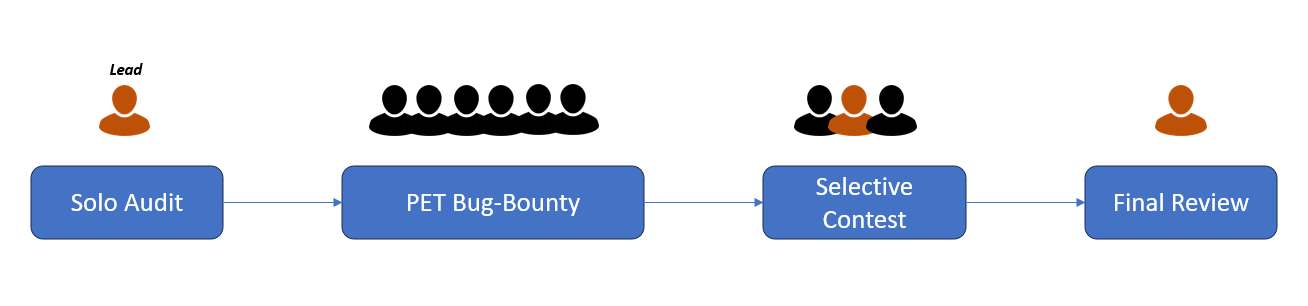
\includegraphics[width=12cm]{img/phases}
  \caption{Phases of the Diverge-Converge MPA}
  \label{fig:galaxy}
\end{figure}

The name \emph{\textbf{Diverge-Converge}} is inspired by the fact that
the audit process starts from a single auditor and diverges into a
public bug bounty, then converges back to a small group of auditors and
finally to a single auditor.

\subsubsection{ Objectives of the Proposed
Model}\label{412-objectives-of-the-proposed-model}

The Diverge-Converge Model emphasizes the following objectives:

\begin{itemize}
\item
  \textbf{Top-Tier Engagement}: The model aims to engage top-tier
  auditors in the whole process by incentivizing them with a fixed
  percentage of the reward pool. This engagement is crucial as it
  ensures the audit is conducted by auditors with relevant domain
  knowledge and experience.
\item
  \textbf{Many Eyes}: The model aims to involve many auditors in the
  audit process via the public bug bounty, increasing the chances of
  identifying vulnerabilities.
\item
  \textbf{Optimized Participation}: The model also aims to provide
  enough incentives for all participants and optimize
  auditors\textquotesingle{} participation. To maximize auditor
  incentives, the model aims to minimize the number of actually rewarded
  participants involved in each phase while achieving top-tier
  engagement and many eyes. This not only increases the rewards for
  auditors but also reduces the turnaround time of the audit.
\item
  \textbf{Long-Term Engagement}: The model aims to support establishing
  a long-term engagement between the client and the lead auditor by
  engaging the lead auditor in all phases. This long-term relationship
  benefits both parties, as the lead auditor gains a deeper
  understanding of the protocol, while the client can leverage the
  auditor\textquotesingle s expertise and experience in future audits.
\item
  \textbf{Information Transfer}: While the model implies a competitive
  spirit amongst auditors, it also enforces a spirit of collaboration
  and knowledge sharing by facilitating the transfer of information from
  one phase to the next, ensuring that all relevant information is
  passed on to the next. The lead auditor is \textbf{required} to share
  the line-by-line comments and walkthrough explanation of the findings
  with the public auditors. The codebase is open to the public through
  the whole process and findings are published as soon as they are
  identified in the first two phases.
\end{itemize}

\subsection{ Roles and Terminology}\label{42-roles-and-terminology}

The Diverge-Converge Model engages several roles.

\begin{itemize}
\tightlist
\item
  \textbf{Client}: The individual or organization that owns the protocol
  and commissions the audit. The client bears the audit cost (reward
  pool).
\item
  \textbf{Lead Auditor}: The individual or organization involved in all
  audit phases. The lead auditor is responsible for conducting a
  comprehensive audit and producing an audit report and a system
  analysis report in the first phase. The lead auditor is also
  responsible for sharing the line-by-line comments and walkthrough
  explanations of the findings with the community auditors. A fixed
  percentage of the reward pool highly incentivizes the lead auditor.
  The lead auditor is also involved across all phases and the dynamic
  structure of the reward pool and audit score incentivize the lead
  auditor to identify more vulnerabilities continuously.
\item
  \textbf{Bounty Hunter}: The individual or organization participating
  in the bug bounty. The bug bounty is open to all, with no limit on
  participant numbers. The lead auditor and bounty hunters are
  implicitly in competition, given the dynamic allocation of the reward
  pool based on findings. Valid findings are rewarded if not identified
  in previous phases and epochs.
\item
  \textbf{Contestant}: The individual or organization participating in
  the selective competition. A small group of auditors, typically 3-5
  including the lead auditor, are chosen as contestants based on their
  performance in previous phases and score. All valid submissions in
  this time-boxed competition are rewarded regardless of the
  duplication.
\item
  \textbf{Judge}: The individual or organization that evaluates the
  findings from all phases. The judge, chosen from a reputable group in
  the Web3 space, is incentivized by a fixed percentage of the reward
  pool.
\item
  \textbf{Host}: The individual or organization overseeing the audit
  process. The host sets up the audit process and ensures its timely
  completion. A fixed fee on top of the reward pool incentivizes the
  host. It is worth noting that the Host holds the final decision-making
  power in the audit process.
\end{itemize}

The Diverge-Converge Model also involves several terms.

\begin{itemize}
\item
  \textbf{Protocol Difficulty}: Based on subjective estimation and the
  SLOC and complexity defined by
  \href{https://marketplace.visualstudio.com/items?itemName=tintinweb.solidity-metrics}{\texttt{solidity-metrics}},
  the Host decides the difficulty score ranging in 0 \textasciitilde{}
  1.
\item
  \textbf{Exploit Score}: A measure representing the implicit audit
  quality. The exploit score is computed based on the protocol
  difficulty, the number of findings, the severity, and the phase of the
  findings.

  The severity of the findings is categorized into three levels: High
  Risk, Medium Risk, and Low Risk. The Judge determines the
  findings\textquotesingle{} severity. Note that we
  don\textquotesingle t include Gas saving findings but an additional
  phase can be added to the end of Phase 3 according to the
  protocol\textquotesingle s preference. See the "Additional Phases"
  section for more details.

  Severity points are given as High Risk: 10 points, Medium Risk: 2
  points, Low Risk: 0.1 point. Phase factor is applied as Phase 1: 0.7x,
  Phase 2: 1x, Phase 3: 1x.

  The idea behind the points by severity is we value the ability to find
  severe ones rather than not impactful ones. The idea behind the points
  by phase is it would be easier to find bugs at an early phase than at
  a later phase.

  The final exploit score is calculated as follows:
  \(ES=C_p*C_d*(N_H*10+N_M*3+N_L)\), where \(C_p\) and \(C_d\) represent
  the phase factor and protocol difficulty.

  \emph{Example}. If an auditor found H3 M2 L10 in phase 1 and the
  difficulty is 0.8, the exploit score will be
  \(0.7*0.8*(3*10+2*3+0.1*10)=20.72\).
\item
  \textbf{Lead Performance Score}: A measure representing the
  performance of the lead auditor. Calculated based on the lead
  auditor\textquotesingle s exploit score (\(ES_L\)) ratio to the other
  auditors\textquotesingle{} exploit score(\(ES_P\)) for all phases.
  After the audit, the lead performance score is calculated as
  \(LS_P=ES_L/ES_P\), capped to {[}0, 2{]}. The lead performance score
  is used to update the auditor score for the lead auditor.
\item
  \textbf{Lead Collaboration Score}: A measure representing the
  collaboration of the lead auditor. The Host evaluates the lead
  auditor\textquotesingle s collaboration level based on the
  line-by-line comments and walkthrough explanation of the findings
  shared with the public auditors. A score \(LS_C\) ranging in
  -10\textasciitilde10 is given to the lead auditor based on the
  evaluation and the score is included in the final audit score of the
  lead auditor.
\item
  \textbf{Auditor Score}: A measure representing the
  auditor\textquotesingle s expertise and experience used to select the
  lead auditor and the contestants. When all phases are finished,
  exploit scores are calculated for all auditors involved in the
  process, and the performance and collaboration scores are calculated
  for the lead auditor.

  Finally, the auditor score is updated as follows:
  \(AS = AS + ES * (LS_P-1) + LS_C\) for the lead auditor
  \(AS = AS + ES\) for other auditors.

  We note that the performance score can increase and decrease the
  auditor score for the lead auditor because \(LS_P\) is capped to {[}0,
  2{]}.
\end{itemize}

\textbf{NOTE} All formulas and parameters are only for illustration
purposes and are not backed by any data. These need to go through actual
experiments and be tuned.

\subsection{ Phases in Detail}\label{43-phases-in-detail}

\subsubsection{ Phase 1: Traditional Audit by Lead
Auditor}\label{431-phase-1-traditional-audit-by-lead-auditor}

\paragraph{Inputs}\label{inputs}

The Protocol team should provide the source code repository access along
with all supportive documentation (papers, manuals, diagrams, etc.) that
could be helpful for the audit. All the inputs are also open to the
public to allow the public auditors to access them as early as possible.

\paragraph{Duration}\label{duration}

The lead auditor provides the Host with an initial estimation of the
necessary duration for this phase. The duration tends to be a tight
estimate as the next phase will have the same duration, while the lead
auditor can win the dynamic pool if he outperforms the public auditors.
This estimated duration is denoted as \(L_P\). The Host decides the
duration based on the protocol\textquotesingle s complexity and the lead
auditor\textquotesingle s estimation. Note that this duration estimation
is vital, as it affects the total cost of the audit and is usually
determined during the negotiation between the Client and the Host.

\paragraph{Execution}\label{execution}

The first phase is a traditional audit by a lead auditor, who could be
an individual or an audit firm. The selection of a lead auditor is based
on their expertise and experience, generally represented as an Auditor
Score. However, the Host can also consider other factors such as the
auditor\textquotesingle s availability and the Client\textquotesingle s
preference.

The lead auditor, engaged in all the phases and playing a vital role in
the audit process, is heavily incentivized with a fixed guaranteed
percentage of the reward pool.

In this phase, the lead auditor\textquotesingle s responsibility is to
conduct a comprehensive audit, producing an audit report and a system
analysis report. The audit process is similar to a traditional audit
model, with the protocol development team involved to assist the lead
auditor in understanding the protocol.

Due to the dynamic structure of the reward pool, the lead auditor is
heavily incentivized to conduct a thorough audit, as the more
vulnerabilities left undiscovered, the lesser the reward will be.
Furthermore, the lead auditor\textquotesingle s performance score
affects the final auditor score, encouraging them to uncover as many
issues as possible.

The entire audit process should be transparent, with findings accessible
to anyone as soon as they are identified. This allows the protocol
development team to begin mitigation immediately as well.

Once the audit is complete, the lead auditor must deliver the Audit
Report V1.0, which contains all the findings and recommended mitigation
steps. The protocol team must address all findings (either fix or
acknowledge them) and provide the Audit Report V1.1, containing all
responses to the lead auditor. The lead auditor checks the mitigation
comments from the protocol and publishes the Audit Report V1.2 with his
responses to all comments. At this point, phase 1 of the audit is
concluded. The lead auditor must also provide an initial system analysis
report, System Analysis Report V1, which describes the protocol from a
security perspective.

Furthermore, the lead auditor must share the line-by-line comments and
walkthrough explanations of the findings with the public auditors. This
facilitates the transfer of information from one phase to the next,
ensuring that all relevant information is passed on to the next phase.
It is worth noting that the lead auditor might have conflicts of
interest in sharing the information with the public auditors, but the
Host can enforce this requirement by contract and utilizing the
collaboration score.

\paragraph{Judging}\label{judging}

The Judge decides the validity and severity of the findings. The Host
may assist in triaging the findings and aiding the Judge in
decision-making if necessary. Notably, neither of the protocol team nor
the lead auditor is the final decision maker. The judging is done in
parallel with the audit process and the findings are published as soon
as they are identified.

\paragraph{Outputs}\label{outputs}

The outputs of this phase include:

\begin{itemize}
\tightlist
\item
  Audit Report V1.2 The report contains all findings and recommendations
  from the lead auditor.
\item
  System Analysis Report V1 The lead auditor is responsible for writing
  a brief system analysis report describing the protocol from a security
  perspective.
\item
  Repository with all comments from the lead auditor Auditors usually
  leave comments to facilitate their understanding and mark the process.
  This is a valuable asset that can significantly assist other auditors.
  The lead auditor is required to leave comments in a kind of standard
  format to help other auditors.
\item
  Video recording of the protocol walkthrough/brainstorm/QA by the lead
  auditor Once the initial audit report V1.0 is delivered, the Host
  arranges a session in which the lead auditor explains the protocol and
  answers questions from other auditors if any. This session is recorded
  and published to assist other auditors in subsequent phases.
\end{itemize}

\subsubsection{ Phase 2: Public Epochal Time-Boxed Bug
Bounty}\label{432-phase-2-public-epochal-time-boxed-bug-bounty}

\paragraph{Inputs}\label{inputs-1}

All outputs from Phase 1 are transferred to Phase 2. A communication
channel is also established between the protocol team and the public
auditors to facilitate dialogue.

\paragraph{Duration}\label{duration-1}

This phase is a public epochal time-bound bug bounty (PET Bug Bounty).
The duration is typically the same as the duration allotted to the lead
auditor, ensuring that the public auditors have ample time to review the
protocol and identify vulnerabilities. As they begin with the lead
auditor\textquotesingle s comments, walkthrough explanation, and the
audit report, this time is expected to be sufficient. Furthermore, the
codebase is open to the public from the beginning of Phase 1, allowing
the public auditors to access it earlier. We denote the bounty duration
as \(L_B\) and by default, we assume \(L_B = L_P\). The Host can adjust
the bounty duration if necessary according to various factors such as
the protocol\textquotesingle s complexity.

\paragraph{Execution}\label{execution-1}

Any public auditor can participate in this phase without any participant
limit.

Unlike other public bug bounty models, this phase is strictly time-boxed
and consists of multiple epochs, each lasting 8\textasciitilde24 hours.
The duration of each epoch is determined by the Host, with the default
assumption of 8 hours. The Host can adjust the epoch duration if
necessary.

Duplicate submissions are permitted within an epoch, but a later epoch
won\textquotesingle t reward a bug already submitted in a previous
epoch. The quality rating (granted by the Judge) is used to determine
the reward for duplicate submissions within a single epoch. The reason
for allowing duplicates within an epoch is to encourage more hunters to
submit their findings because they have a chance to win the reward even
if they are not the first to find the bug. Leveraging the quality rating
to "sort" the findings ensures that the submissions are high quality and
the reward is allocated to the most deserving hunter.

To prevent premature disclosure, hunters can opt for a "hash submission"
where they will initially submit just the hash of their findings and the
full details are open to the judges only after a block concludes. The
findings are published as soon as possible to help hunters avoid
duplicate submissions.

The judgment process is transparent and allows for an appeal from
auditors if they disagree with the judges. To aid judges in
understanding the findings, auditors are strongly encouraged to provide
a proof of concept (PoC). In this phase, only the High and Medium risk
findings are considered.

Valid findings are published on the finding board as soon as they are
identified, allowing the protocol team to initiate mitigation
immediately.

The lead auditor is also involved in this phase and is incentivized to
continue exploring the protocol to find more vulnerabilities. Although
the lead auditor\textquotesingle s findings will not be rewarded as they
are considered "known issues from Phase 1", their score will be updated
accordingly. The dynamic structure of the reward pool and audit score
incentivizes the lead auditor to identify more vulnerabilities.

By the dynamic structure of the reward pool, the public auditors are
incentivized enough to conduct a thorough audit. On the other hand,
there are likely few vulnerabilities left undiscovered assuming the lead
auditor has done an excellent job. This gives a chance for the public
auditors to win a high reward with a single submission.

Once the bounty period is over (all epochs are finished and judged), the
Host delivers the Audit Report V2.0, containing all findings and
recommended mitigation steps. The protocol team must address all
findings (either fix or acknowledge them), and deliver the Audit Report
V2.1, containing all responses to the findings.

This phase does \textbf{NOT} have a mitigation review process; this will
be conducted in the next phase.

\textbf{NOTE 1:} Public auditors are encouraged to submit any findings
that arise after the bounty period. These findings will be reviewed at
the end of Phase 3 and, if not covered elsewhere, will be rewarded as
part of the contest pool.

\textbf{NOTE 2:} The term PET Bug Bounty can be replaced with other
terms such as "Public Epochal Contest" because it is essentially a
generalization of the existing bug bounty models and public contest
models. If the epoch duration is the same as the whole duration, it is
equivalent to a public contest. If the epoch duration is zero and the
whole duration is infinite, it equals a traditional bug bounty.

\paragraph{Judging}\label{judging-1}

The Judge determines the validity and severity of the findings. The Host
may assist in triaging the findings and aiding the Judge in
decision-making if necessary. Notably, neither the protocol team nor the
lead auditor is the final decision maker. The Judge gets access to the
full details of the findings of the previous epoch only after the epoch
concludes. The judging is done in parallel with the bounty process and
the findings are published as soon as they are identified.

\paragraph{Outputs}\label{outputs-1}

The output of this phase is the Audit Report V2.0, containing all
findings.

\subsubsection{ Phase 3: Selective
Competition}\label{433-phase-3-selective-competition}

This phase is primarily focused on reviewing the mitigations of all the
findings from the previous phases. Any new vulnerabilities introduced
during the mitigation process should be identified in this phase.

\paragraph{Inputs}\label{inputs-2}

All outputs from Phases 1 and 2 are transferred to Phase 3.

A small group of auditors, typically 3-5 including the lead auditor, are
chosen as contestants based on their performance in the Phase 2 and
their auditor score.

A new communication channel is opened between the protocol team and the
contestants.

\paragraph{Duration}\label{duration-2}

This phase is a time-bound selective competition. The Host, in
consultation with the lead auditor, estimates the necessary duration for
this phase, typically recommended to be between 3 to 7 days. We denote
the contest duration as \(L_C\), with a default assumption of
\(L_C = 5\). The Host can adjust the contest duration if necessary.

\paragraph{Execution}\label{execution-2}

The chosen contestants review the mitigated protocol and aim to find any
additional vulnerabilities. The findings are not limited to mitigated
issues, and contestants are encouraged to find any vulnerabilities in
the protocol. All severity levels are considered in this phase.

The lead auditor continues their involvement in this phase and is
incentivized to find more vulnerabilities. The lead
auditor\textquotesingle s findings are rewarded as part of the contest
pool and will affect their performance score.

After the contest concludes, a judging period commences during which the
judges review all findings from the contestants and the lead auditor.
They determine the validity and severity of the findings. The judging
process is transparent, allowing auditors to appeal their findings.

Once judging begins, any additional submissions (after the public bounty
time has concluded) are published, and the contestants collaborate with
the judges to evaluate these findings. Contestants are interested in
this process as these findings will influence the final distribution of
the reward pool.

Once judging concludes, the Host delivers the Audit Report V3.0,
containing all findings and recommended mitigation steps. The protocol
team must address all findings (either fix or acknowledge them), and
deliver the Audit Report V3.1, containing all responses to the findings.
The lead auditor then delivers Audit Report V3.2, containing responses
to mitigation comments.

\paragraph{Judging}\label{judging-2}

The Judge determines the validity and severity of the findings. The
judging is started after the contest concludes and the findings are
published. Judges are incentivized to complete the judging process on
time. We denote the judging duration as \(L_J\), with a default
assumption of \(L_J = 3\). The Host can adjust the judging duration if
necessary. It\textquotesingle s noteworthy that this contest is very
likely to involve only a smaller number of findings.

\paragraph{Outputs}\label{outputs-2}

The output of this phase is the Audit Report V3.2, containing all
findings and comments regarding the fixes.

\subsubsection{ Phase 4: Final
Review}\label{434-phase-4-final-review}

The Host reviews the entire process and generates the final audit
process report. The lead auditor is encouraged to revise the system
analysis report based on a deeper understanding of the protocol acquired
during the process. We denote the duration of this phase as \(L_F\) with
a default assumption of \(L_F = 2\).

\subsection{ Reward Pool Structure}\label{44-reward-pool-structure}

The Client bears the cost of the audit, referred to as the reward pool,
and the Host organizes the structure of the reward pool. The reward pool
structure is dynamically designed to incentivize the auditors and
adequately maximize the quality of audits. The Host is assumed to charge
a fixed fee in addition to the reward pool.

\begin{figure}[htp]
  \centering
  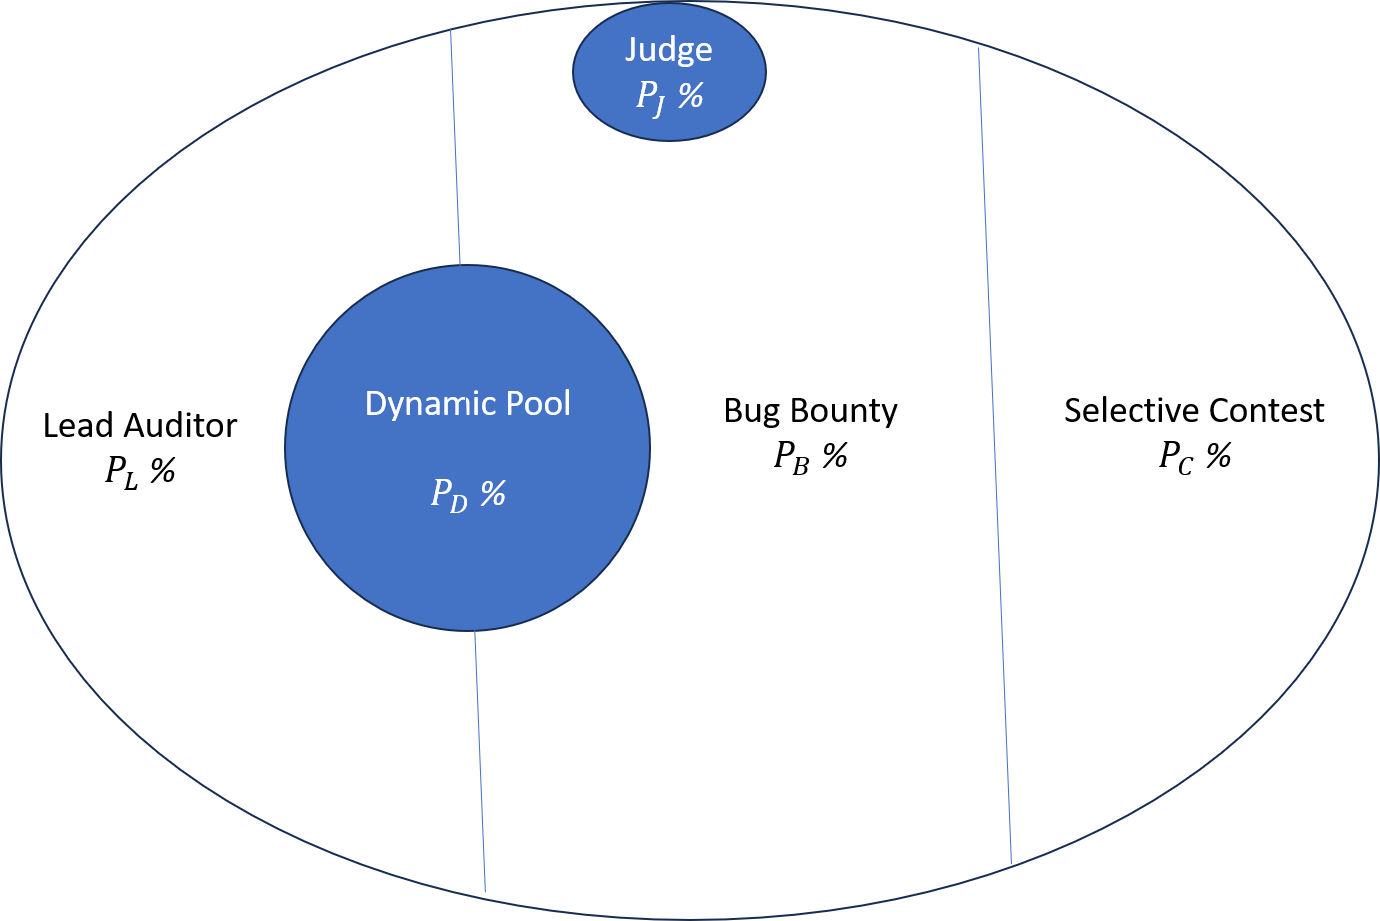
\includegraphics[width=10cm]{img/pool}
  \caption{Reward Pool of the Diverge-Converge MPA}
  \label{fig:galaxy}
\end{figure}

\begin{itemize}
\tightlist
\item
  \textbf{Lead Auditor}: The lead auditor is greatly incentivized with a
  fixed guaranteed percentage (\(P_L\%\)) of the reward pool. It is
  recommended that \(20 \leq P_L < 50\).
\item
  \textbf{Bug Bounty}: A fixed percentage (\(P_B\%\)) of the reward pool
  is reserved for the bug bounty and is used to incentivize the public
  to identify vulnerabilities in the protocol \textbf{AFTER} the
  mitigation of findings from the first phase. It is recommended that
  \(P_L \leq P_B < 50\). The bug bounty pool is distributed to the lead
  auditor if no vulnerabilities are found during the bug bounty phase.
\item
  \textbf{Dynamic Pool}: A fixed percentage (\(P_D\%\)) of the reward
  pool is reserved as a dynamic pool. This pool will be rewarded to the
  lead auditor or the bounty hunters based on the lead
  auditor\textquotesingle s performance. It is recommended that
  \(P_D = 50 - P_L\).
\item
  \textbf{Selective Competition Pool}: A fixed percentage (\(P_C\%\)) of
  the reward pool is reserved for the selective competition pool and is
  used to incentivize the contestants to identify vulnerabilities in the
  protocol \textbf{AFTER} the mitigation of findings from the second
  phase. It is recommended that \(10 \leq P_C \leq 15\). As this phase
  allows for LOW risks, this pool will likely always be distributed to
  the contestants.
\item
  \textbf{Judge}: The judge is involved in all phases and incentivized
  by a fixed guaranteed percentage (\(P_J\%\)) of the reward pool. It is
  recommended that \(5 \leq P_J \leq 15\).
\end{itemize}

\subsubsection{Default Pool Structure}\label{default-pool-structure}

The default pool structure is assumed to be \(P_L=30\), \(P_B=30\),
\(P_D=20\), \(P_C=10\), \(P_J=10\).

\subsection{ Process Overview}\label{45-process-overview}

The overall process is as follows, assuming the default pool structure.

\begin{longtable}[]{@{}lllll@{}}
\toprule\noalign{}
Phase & Reward & Participant & Duration & Result \\
\midrule\noalign{}
\endhead
\bottomrule\noalign{}
\endlastfoot
Traditional Audit by Lead Auditor & 30\% (+20\%) & Lead Auditor &
\(L_P\) days & Audit Report V1.2, System Analysis Report V1, Commented
Repo, Walkthrough Video \\
PET Bug Bounty & 30\% (+20\%) & Public & \(L_B\) days & Audit Report
V2.0 \\
Selective Contest & 10\% & Selected Auditors & \(L_C\) days & Audit
Report V3.1 \\
Final Review & 0 & Lead Auditor & \(L_F\) days & Final Audit Report,
Final System Analysis Report \\
\end{longtable}

\subsection{ Estimation of Time and
Cost}\label{46-estimation-of-time-and-cost}

The entire process\textquotesingle s cost can be estimated starting from
the lead auditor\textquotesingle s price and engagement duration.

As previously mentioned, the lead auditor estimates the duration for
Phase 1 as \(L_P\) days, and the Host sets the time for the remaining
phases as \(L_B\), \(L_C\), and \(L_F\) days. Due to the dynamic pool
structure, the lead auditor is motivated to estimate the duration
accurately.

Let\textquotesingle s assume the lead auditor\textquotesingle s daily
cost for 100\% dedication is \(C_L\).

We estimate the lead auditor\textquotesingle s dedication for each
phase: \(D_P = 100\%\), \(D_B = 50\%\), \(D_C = 100\%\), \(D_F = 0\%\).

The total cost for the lead auditor can be estimated as
\(C_L * (L_P * D_P + L_B * D_B + L_C * D_C) = C_L * (L_P + L_B/2 + L_C)\).

Assuming the lead auditor outperforms the public auditors, the lead
auditor will receive \(P_L + P_D\%\) of the reward pool (50\% for the
default structure). So, we can estimate the entire reward pool (i.e.,
the total cost) as \(C_L * (L_P + L_B/2 + L_C) * 100 / (P_L + P_D)\).

The total turnaround time can be estimated as
\(L_P + L_B + L_C + L_J + L_F\) days.

\emph{Example} Assuming the lead auditor\textquotesingle s engagement
cost is \(C_L = 2000\$\) per day and he estimated the duration for Phase
1 as \(L_P = 10\) days. With the default pool structure and the duration
of other phases as \(L_B = L_P = 10\), \(L_C = 5\), the total cost would
be \(2000 * (10 + 10/2 + 5) * 100 / (30 + 20) = \$80,000\), and the
complete turnaround would be approximately a month probably including
the mitigation turnaround.

\subsection{ Additional Phases}\label{47-additional-phases}

The Diverge-Converge model is flexible and can be adjusted to suit the
protocol team\textquotesingle s needs. For instance, the Client may add
a phase to the audit process to address gas optimization issues. The
Client might also want to have another round of review from a reputable
audit firm after Phase 3 to get advice on the system architecture and
deployment. Theoretically, the more rounds of review, the better the
audit quality. However, the cost of the audit will increase accordingly.
The Client should carefully consider the trade-off between price and
quality.

\subsection{ Summary}\label{48-summary}

In this section, we proposed the Diverge-Converge Multi-Phase Audit
Model, which strives to maximize audit quality by incentivizing auditors
appropriately and ensuring the protocol codebase undergoes at least
three audit phases. The proposed model has several advantages:

\begin{itemize}
\tightlist
\item
  The protocol codebase undergoes at least three audit phases. This
  sequence, connected via a set of incentives and disincentives, is not
  equivalent to three separate audits; instead, it creates a potent
  competition among auditors.
\item
  The model ensures audit quality by properly incentivizing auditors. In
  particular, the lead auditor is highly incentivized, securing top-tier
  engagement critical for high-quality audits. Moreover, the dynamic
  reward pool structure also incentivizes public auditors. Depending on
  performance, a single public auditor could earn more than the lead
  auditor theoretically. The innovative reward pool structure is a
  crucial strength of the model to achieve top-tier engagement and "many
  eyes".
\item
  The model is efficient. Transferring all information from one phase to
  the next increases audit process efficiency. Findings are published
  immediately, enabling the protocol team to start mitigation
  immediately.
\item
  The model\textquotesingle s core is transparent and fair. Auditors can
  communicate with each other, the protocol team, and the judges
  throughout the audit.
\item
  The lead auditor\textquotesingle s extended engagement helps the
  protocol team build a long-term relationship with them.
\item
  The flexible model can be adjusted to suit the protocol
  team\textquotesingle s needs. For instance, Phase 2 could be performed
  by a limited number of auditors instead of a public community. An
  individual auditor or an audit firm could perform phase 1.
\end{itemize}

\section{ Conclusion}\label{5-conclusion}

This paper presents an overview of existing audit models in Web3,
proposing a new, innovative model known as the Diverge-Converge
Multi-Phase Model. This model is crafted to maximize the quality of
audits, a critical aspect in the Web3 space. By strategically
incentivizing auditors and ensuring that the protocol codebase goes
through at least three comprehensive auditing phases, the model aims to
enhance audit quality significantly.

The unique strength of the Diverge-Converge Model lies in its ability to
foster robust competition among auditors, backed by a dynamic reward
pool structure. This structure ensures the engagement of top-tier
auditors and encourages their continuous involvement throughout the
process. Furthermore, the model emphasizes transparency, promoting
efficient communication among auditors, the protocol team, and judges.

The Diverge-Converge Multi-Phase Audit Model introduces a novel approach
to auditing in the Web3 space, addressing the possible shortcomings of
existing models while presenting its unique advantages. As Web3
continues to grow and evolve, this model could serve as a new standard,
guiding the way toward more effective and high-quality audits. Further
experiments and implementations of this model will provide more insights
and potential enhancements, contributing to the continuous improvement
and refinement of auditing practices in the Web3 space.

\section{ Acknowledgments}\label{6-acknowledgments}

We sincerely thank the entire \href{https://www.cyfrin.io/}{Cyfrin} team
for their invaluable contributions and advice. Their insights and
expertise were instrumental in refining and enhancing our ideas.
Additionally, special thanks to
\href{https://twitter.com/Montyly}{Josselin Feist} from
\href{https://www.trailofbits.com/}{Trail of Bits} and
\href{https://twitter.com/tinchoabbate}{Tincho} for reviewing the paper
and offering valuable insights and advice.

\section{ References}\label{7-references}

\begin{itemize}
\tightlist
\item
  {[}1{]}
  \href{https://www.youtube.com/watch?v=_Yul_fHUjr8&list=PL5r4vTR0gHj5JL62S9R0umY64ue6mfQhd&index=43}{DeFi
  Security Summit 2023 - Session 16: Audits Conventional vs Community
  Panel}
\item
  {[}2{]} \href{https://code4rena.com/}{Code4rena}
\item
  {[}3{]} \href{https://sherlock.xyz/}{Sherlock}
\item
  {[}4{]} \href{https://app.hats.finance/}{Hats.finance}
\item
  {[}5{]} \href{https://spearbit.com/}{SpearbitDAO}
\item
  {[}6{]} \href{https://auditone.io/}{AuditOne}
\item
  {[}7{]}
  \href{https://marketplace.visualstudio.com/items?itemName=tintinweb.solidity-metrics}{Solidity
  Metrics} by \href{https://www.consensys.net/}{Consensys}
\item
  {[}8{]}
  \href{https://www.chainalysis.com/blog/2022-biggest-year-ever-for-crypto-hacking/}{Report
  2022} by \href{https://www.chainalysis.com/}{Chainalysis}
\end{itemize}

\end{document}